\documentclass[12pt]{beamer}
\usepackage{luatexja}
\usepackage{amsmath}
\usepackage{grffile}
\usefonttheme[onlymath]{serif}
\setbeamertemplate{navigation symbols}{}
\title{PRML 3 線形回帰モデル}
\institute{大阪PRML読書会}
\date{2014年8月31日}
\begin{document}

\renewcommand{\l}{\left}
\renewcommand{\r}{\right}
\newcommand{\f}{\frac}
\newcommand{\p}[2]{\frac{\partial #1}{\partial #2}}

\newcommand{\TT}{{\rm T}}
\newcommand{\ML}{{\rm ML}}
\newcommand{\e}{{\rm \bf e}}
\renewcommand{\t}{{\rm \bf t}}
\renewcommand{\v}{{\rm \bf v}}
\newcommand{\w}{{\rm \bf w}}
\renewcommand{\x}{{\rm \bf x}}
\newcommand{\y}{{\rm \bf y}}
\newcommand{\bphi}{\boldsymbol \phi}
\newcommand{\bvphi}{\boldsymbol \varphi}
\newcommand{\bPhi}{{\rm \bf \Phi}}
\newcommand{\E}{{\mathbb{E}}}
\newcommand{\N}{{\cal N}}
\newcommand{\A}{{\rm \bf A}}
\newcommand{\I}{{\rm \bf I}}
\newcommand{\T}{{\rm \bf T}}
\newcommand{\W}{{\rm \bf W}}
\newcommand{\X}{{\rm \bf X}}
\renewcommand{\tt}{{\bf \mathsf{t}}}
\newcommand{\yy}{{\bf \mathsf{y}}}
\renewcommand{\S}{\mathcal{S}}

\maketitle

\begin{frame}
  \frametitle{目次}
  \setcounter{tocdepth}{3}
  \tableofcontents
\end{frame}

\section{3 線形回帰モデル}

\subsection{導入}

\begin{frame}
  \frametitle{導入}
  回帰問題に対する二つのアプローチ
  \begin{itemize}
  \item
    予測関数\(y(\x)\)を構成する。
  \item
    条件付き確率分布関数\(p(t|\x)\)を構成する。\\
    その分布の下で期待損失を最小化するように \\
    \(\x\)に対する\(t\)を決定する。
  \end{itemize}
\end{frame}

\subsection{3.1 線形基底関数モデル}

\begin{frame}
  \frametitle{線形基底関数モデル}
  一般形
  \begin{align*}
    y(\x,\w) = & w_0 + \sum_{j=1}^{M-1} w_j \phi_j(\x) \\
             = & \sum_{j=0}^{M-1} w_j \phi_j(\x) \\
             = & \w^\TT \bphi(\x) \\
  \end{align*}
  \begin{align*}
    \text{ where }
    & \phi_j(\x) : 基底関数 \\
    & \phi_0(\x) = 1 : ダミーの基底関数 \\
    & \bphi = (\phi_0,...,\phi_{M-1})^\TT \\
    & \w = (w_0,...,w_{M-1})^\TT \\
  \end{align*}
\end{frame}

\begin{frame}
  \frametitle{線形基底関数モデル}
  \begin{figure}
    \centering
    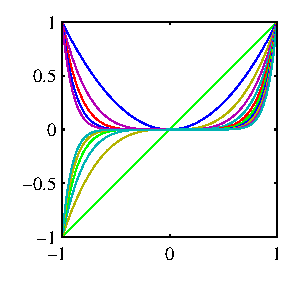
\includegraphics[width=3.5cm]{Figure3.1a.pdf}
    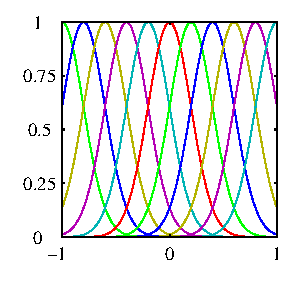
\includegraphics[width=3.5cm]{Figure3.1b.pdf}
    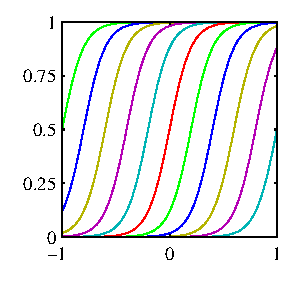
\includegraphics[width=3.5cm]{Figure3.1c.pdf}
  \end{figure}
\end{frame}

\subsubsection{3.1.1 最尤推定と最小二乗法}

\begin{frame}
  \frametitle{最尤推定と最小二乗法}
  目標変数\(t\)が、決定論的な関数\(y(\x,\w)\)とガウスノイズの和で与えられると仮定する。
  \begin{align*}
    t = y(\x,\w) + \epsilon && \text{where} && p(\epsilon|\beta) = \N(\epsilon|0,\beta^{-1})
  \end{align*}
  これは以下と等価である。
  \begin{align*}
    p(t|\x,\w,\beta) = & \N(t|y(\x,\w),\beta^{-1})
  \end{align*}
\end{frame}

\begin{frame}
  \frametitle{最尤推定と最小二乗法}
  決定段階 \\[2ex]
  損失関数として二乗損失関数を仮定すると、 \\
  新しい\(\x\)の値に対する最適な予測値は \\
  目標変数の条件付き期待値で与えられる。
  \begin{align*}
    t = \E[t|\x] = \int t p(t|\x) dt
  \end{align*}

  先に仮定した条件付き確率分布を用いると、
  \begin{align*}
    t = & \int t \N(t|y(\x,\w),\beta^{-1}) dt \\
      = & y(\x,\w)
  \end{align*}
  \(t\)は決定論的関数の値として与えられる。
\end{frame}

\begin{frame}
  \frametitle{最尤推定と最小二乗法}
  データ集合
  \begin{align*}
    \X = & (\x_1,...,\x_N)^\TT \\
    \tt = & (t_1,...,t_N)^\TT
  \end{align*}
  尤度関数
  \begin{align*}
    p(\tt|\X,\w,\beta) = & \prod_{n=1}^N \N(t_n|\w^\TT \bphi(\x_n),\beta^{-1})
  \end{align*}
\end{frame}

\begin{frame}
  \frametitle{最尤推定と最小二乗法}
  対数尤度関数
  \begin{align*}
        \ln p(\tt|\w,\beta)
    = & \sum_{n=1}^N \ln \N(t_n|\w^\TT \bphi(\x_n),\beta^{-1}) \\
    = & \sum_{n=1}^N \ln \l[ \l(\f{\beta}{2 \pi}\r)^{1/2}
        \exp\l\{ -\f{\beta}{2} (t_n - \w^\TT \bphi(\x_n))^2 \r\} \r] \\
    = & \f{N}{2} \ln \beta - \f{N}{2} \ln 2 \pi - \beta E_D(\w)
  \end{align*}
  ただし
  \begin{align*}
    E_D(\w) = & \f{1}{2} \sum_{n=1}^N \l\{ t_n - \w^\TT \bphi(\x_n) \r\}^2
  \end{align*}
  \(E_D\)は二乗和誤差関数。
\end{frame}

\begin{frame}
  \frametitle{最尤推定と最小二乗法}
  \(\w\)の最尤推定
  \begin{gather*}
    \nabla \ln p(\tt|\w,\beta) = \beta \sum_{n=1}^N \l\{ t_n - \w^\TT \bphi(\x_n) \r\} \bphi(\x_n)^\TT \\
    \begin{aligned}
      0 = & \sum_{n=1}^N t_n \bphi(\x_n)^\TT
          - \w_{\ML}^\TT \l( \sum_{n=1}^N \bphi(\x_n) \bphi(\x_n)^\TT \r) \\
      0 = & \bPhi^\TT \tt
          - \w_{\ML}^\TT \l( \bPhi^\TT \bPhi \r) \\
      \w_{\ML} = & \l( \bPhi^\TT \bPhi \r)^{-1} \bPhi^\TT \tt = \bPhi^\dagger \tt
          \qquad \cdots \text{正規方程式}
    \end{aligned}
  \end{gather*}
  ただし、\(\bPhi\)は計画行列 design matrix。
  \begin{align*}
    \bPhi
    = \l( \begin{array}{c}
      \bphi(\x_1)^\TT \\
      \bphi(\x_2)^\TT \\
      \vdots       \\
      \bphi(\x_N)^\TT
    \end{array} \r)
    = \l( \begin{array}{cccc}
      \phi_0(\x_1) & \phi_1(\x_1) & \cdots & \phi_{M-1}(\x_1) \\
      \phi_0(\x_2) & \phi_1(\x_2) & \cdots & \phi_{M-1}(\x_2) \\
      \vdots       & \vdots      & \ddots & \vdots           \\
      \phi_0(\x_N) & \phi_1(\x_N) & \cdots & \phi_{M-1}(\x_N)
    \end{array} \r)
  \end{align*}
\end{frame}

\begin{frame}
  \frametitle{最尤推定と最小二乗法}
  バイアスパラメータ\(w_0\)の役割
  \begin{align*}
    E_D(\w) = & \f{1}{2} \sum_{n=1}^N \l\{ t_n - w_0 - \sum_{j=1}^{M-1} w_j \phi_j(\x_n) \r\}^2 \\
    \p{}{w_0} E_D(\w) = & - \sum_{n=1}^N \l\{ t_n - w_0 - \sum_{j=1}^{M-1} w_j \phi_j(\x_n) \r\}
  \end{align*}

  \begin{align*}
    w^{\ML}_0 = \overline{t} - \sum_{j=1}^{M-1} w^{\ML}_j \overline{\phi_j}
  \end{align*}

  \begin{align*}
         \overline{t} = & \f{1}{N} \sum_{n=1}^N t_n          & \text{目標値の訓練集合に関する平均} \\
    \overline{\phi_j} = & \f{1}{N} \sum_{n=1}^N \phi_j(\x_n) & \text{基底関数の値の訓練集合に関する平均}
  \end{align*}
\end{frame}

\begin{frame}
  \frametitle{最尤推定と最小二乗法}
  \(\beta\)の最尤推定
  \begin{align*}
    \p{}{\beta} \ln p(\tt|\w,\beta)
    = & \p{}{\beta} \l\{ \f{N}{2} \ln \beta - \f{N}{2} \ln 2 \pi - \beta E_D(\w) \r\} \\
    = & \f{N}{2} \f{1}{\beta} - E_D(\w)
  \end{align*}
  \begin{align*}
    \f{N}{2} \f{1}{\beta_{\ML}} - E_D(\w_{\ML}) = & 0 \\
    \f{1}{\beta_{\ML}} = & \f{1}{N} \sum_{n=1}^N \l\{ t_n - \w_{\ML}^\TT \bphi(\x_n) \r\}^2
  \end{align*}
  ノイズの精度の逆数は、\\
  回帰関数周りでの目標値の残差分散で与えられる。
\end{frame}

\subsubsection{3.1.2 最小二乗法の幾何学}

\begin{frame}
  \frametitle{最小二乗法の幾何学}
  各軸が\(t_n\)で与えられる\(N\)次元空間。
  \begin{description}
  \item[\(\tt=(t_1,...,t_N)^\TT\)] \\
    訓練データ集合の目標値の集合。
  \item[\(\bvphi_j=(\phi_j(\x_1),...,\phi_j(\x_N))^\TT\)] \\
    訓練データ集合の基底関数の値の集合。\\
    \(\bvphi_j\)は\(\bPhi\)の列ベクトル。\(\bphi(\x_n)^\TT\)は行ベクトル。
    \(M\)個の\(\bvphi_j\)は\(M\)次元の線形部分空間\(\S\)を張る。
  \item[\(\yy=(y(\x_1,\w),...,y(\x_N,\w))^\TT\)] \\
    目標値の予測値の集合。\\
    \(\yy\)は\(\bvphi_j\)の線形結合なので\(\S\)上にある。
  \end{description}
  \begin{align*}
     \yy = & (\bphi(\x_1)^\TT \w,...,\bphi(\x_N)^\TT \w)^\TT \\
         = & (\bphi(\x_1)^\TT,...,\bphi(\x_N)^\TT)^\TT \w \\
         = & \bPhi \w \\
         = & (\bvphi_0,...,\bvphi_{M-1}) \w \\
\  \end{align*}
\end{frame}

\begin{frame}
  \frametitle{最小二乗法の幾何学}
  \begin{figure}
    \centering
    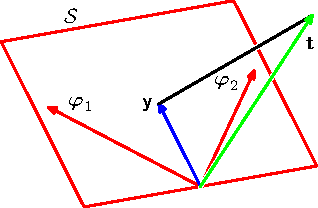
\includegraphics[width=7cm]{Figure3.2.pdf}
  \end{figure}
  \begin{align*}
    \sum_{n=1}^N \l\{ t_n - \w^\TT \bphi(\x_n) \r\}^2 = \| \tt - \yy \|^2
  \end{align*}
\end{frame}

\begin{frame}
  \frametitle{演習3.2}
  [定義] \(\v'\)が\(\v\)の\(\S\)への正射影である。\\
  ただし、\(\S\)は基底ベクトル\(\{\e_j\}\)が張る空間。\(\A = (\e_1,...,\e_M)\)。
  \begin{enumerate}
  \item \(\v'\)が\(\S\)上にある。\\
    \(\exists \w. \v' = \sum_j \e_j w_j \Leftrightarrow ∃\w. \v' = \A \w\)
  \item \(\v-\v'\)が\(\S\)と直交する。\\
    \(\forall j.\e_j (\v - \v') = 0 \Leftrightarrow \A^\TT (\v - \v') = 0\)
  \end{enumerate}
   \\

  \(\v' = \bPhi (\bPhi^\TT \bPhi)^{-1} \bPhi^\TT \v\)と置く。\\
  \begin{enumerate}
  \item \(\w = (\bPhi^\TT \bPhi)^{-1} \bPhi^\TT \v\)と置けばただちに成り立つ。\\
  \item
    \(\begin{aligned}[t]
        \bPhi^\TT (\v - \v')
    = & \bPhi^\TT (\v - \bPhi (\bPhi^\TT \bPhi)^{-1} \bPhi^\TT \v) \\
    = & (\bPhi^\TT - \bPhi^\TT \bPhi (\bPhi^\TT \bPhi)^{-1} \bPhi^\TT) \v \\
    = & (\bPhi^\TT - \bPhi^\TT) \v \\
    = & 0
    \end{aligned}\)
  \end{enumerate}
\end{frame}

\begin{frame}
  \frametitle{演習3.2}
  \(\yy\)の定義より
  \begin{align*}
    \yy = & \bPhi \w
  \end{align*}
  \(\w\)の最小二乗解は正規方程式(3.15)により
  \begin{align*}
    \w_{\ML} = (\bPhi^\TT \bPhi)^{-1} \bPhi^\TT \tt
  \end{align*}
  \(\yy\)の最小二乗解は
  \begin{align*}
    \yy_{\ML} = & \bPhi (\bPhi^\TT \bPhi)^{-1} \bPhi^\TT \tt
  \end{align*}
  よって、\(\yy\)の最小二乗解は\\
  \(\tt\)の\(\bPhi\)の列ベクトルが張る多様体\(\S\)への正射影である。
\end{frame}

\subsubsection{3.1.3 逐次学習}

\begin{frame}
  \frametitle{逐次学習}
  確率的勾配降下法 stochastic gradient descent
  \begin{align*}
    \w^{(\tau+1)} = \w^{(\tau)} - \eta \nabla E_n
  \end{align*}
  二乗和誤差関数
  \begin{align*}
    E_n(\w)=\f{1}{2} (t_n - \w^\TT \bphi(\x_n))^2
  \end{align*}
  を用いると
  \begin{align*}
    \w^{(\tau+1)} = \w^{(\tau)} + \eta (t_n - {\w^{(\tau)}}^\TT \bphi(\x_n)) \bphi(\x_n)
  \end{align*}
  最小平均二乗アルゴリズム\\
  least-mean-squares (LMS) algorithm
\end{frame}

\subsubsection{3.1.4 正則化最小二乗法}

\begin{frame}
  \frametitle{正則化最小二乗法}
  正則化された誤差関数
  \begin{align*}
    E_D(\w) & + \lambda E_W(\w) \\
    & E_D(\w) : データに依存する誤差 \\
    & E_W(\w) : 正則化項
  \end{align*}

  二乗和誤差関数 + 二次正則化項
  \begin{align*}
    \f{1}{2} \sum_{n=1}^N \{ t_n - \w^\TT \bphi(\x_n) \}^2 + \f{1}{2} \w^\TT \w
  \end{align*}

  最小化
  \begin{align*}
    \w = (\lambda \I + \bPhi^\TT \bPhi)^{-1} \bPhi^\TT \tt
  \end{align*}
\end{frame}

\begin{frame}
  \frametitle{正則化最小二乗法}
  誤差関数の最小化
  \begin{align*}
    & \nabla \l[ \f{1}{2} \sum_{n=1}^N \{ t_n - \w^\TT \bphi(\x_n) \}^2
      + \f{\lambda}{2} \w^\TT \w \r] \\
    = & - \bPhi^\TT \tt + \w^\TT \bPhi^\TT \bPhi + \lambda \w^\TT \\
    = & - \bPhi^\TT \tt + \w^\TT \bPhi^\TT \bPhi + \w^\TT (\lambda \I) \\
    = & - \bPhi^\TT \tt + \w^\TT ( \lambda \I + \bPhi^\TT \bPhi ) \\
  \end{align*}
\end{frame}

\begin{frame}
  \frametitle{正則化最小二乗法}
  二乗和誤差関数 + \(q\)次正則化項
  \begin{align*}
    \f{1}{2} \sum_{n=1}^N \{ t_n - \w^\TT \bphi(\x_n) \}^2 + \f{\lambda}{2} \sum_{j=1}^M |w_j|^q
  \end{align*}
  \begin{figure}
    \centering
    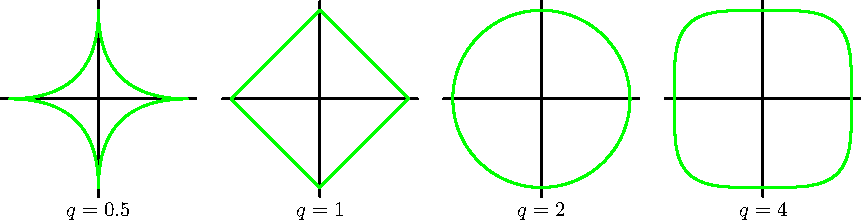
\includegraphics[width=10cm]{Figure3.3.pdf}
  \end{figure}
\end{frame}

\begin{frame}
  \frametitle{正則化最小二乗法}
  \begin{figure}
    \centering
    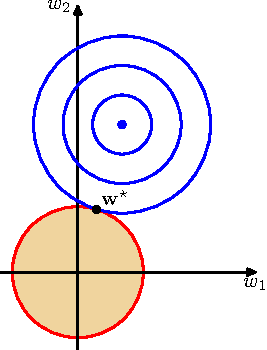
\includegraphics[width=5cm]{Figure3.4a.pdf}
    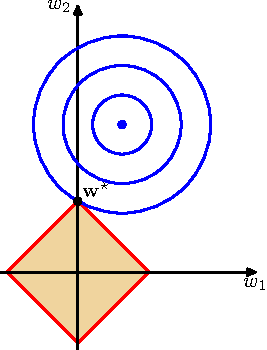
\includegraphics[width=5cm]{Figure3.4b.pdf}
  \end{figure}
\end{frame}

\begin{frame}
  \frametitle{演習3.5}
  制約条件(3.30)は以下のように書き換えられる。
  \begin{align*}
    \sum_{j=1}^M |w_j|^q \leq \eta
    \Leftrightarrow
    -\f{1}{2} \l( \sum_{j=1}^M |w_j|^q - \eta \r) \geq 0
  \end{align*}
  ラグランジュ関数
  \begin{align*}
    L(\w,\lambda) = \f{1}{2} \sum_{n=1}^N \{ t_n - \w^\TT \bphi(\x_n) \}^2
                  + \f{\lambda}{2} \l( \sum_{j=1}^M |w_j|^q - \eta \r) \\
    \text{where} \qquad g(\w) \geq 0 \qquad \lambda \geq 0 \qquad \lambda g(\w) = 0
  \end{align*}
  停留条件
  \begin{alignat*}{3}
    \nabla L(\w,\lambda) = 0 &
    \rightarrow & \text{正則化された誤差関数の最小化と同じ} \\
    \p{}{\lambda} L(\w,\lambda) = 0 &
    \rightarrow & \eta = \sum_{j=1}^M |w_j|^q = \sum_{j=1}^M |w_j(\lambda)|^q
  \end{alignat*}
\end{frame}

\subsubsection{3.1.5 出力変数が多次元の場合}

\begin{frame}
  \frametitle{出力変数が多次元の場合}
  \(\t\)のすべての要素に同じ基底関数を用いたモデル
  \begin{align*}
    \y(\x,\w) = \W^\TT \bphi(\x)
  \end{align*}

  \(\t\)の条件付き分布を等方性ガウス分布と仮定する。
  \begin{align*}
    p(\t|\x,\W,\beta) = \N(\t|\W^\TT \bphi(\x),\beta^{-1} \I)
  \end{align*}
\end{frame}

\begin{frame}
  \frametitle{出力変数が多次元の場合}
  データ集合\(\quad \T = (\t_1,...,\t_N)^\TT\)、\(\X = (\x_1,...,\x_N)^\TT\)\\
  対数尤度関数
  \begin{align*}
      & \ln p(\T|\X,\W,\beta) \\
    = & \sum_{n=1}^N \ln \N(\t_n|\W^\TT \bphi(\x_n),\beta^{-1} \I) \\
    = & \sum_{n=1}^N \ln \l[ \l(\f{\beta}{2 \pi}\r)^{K/2}
        \exp\l\{ -\f{\beta}{2} \| \t_n - \w^\TT \bphi(\x_n) \|^2 \r\} \r] \\
    = & \f{NK}{2} \ln \l( \f{\beta}{2 \pi} \r)
      - \f{\beta}{2} \sum_{n=1}^N \| \t_n - \W^\TT \bphi(\x_n) \|^2
  \end{align*}

  最尤解
  \begin{align*}
    \W_{\ML} = & ( \bPhi^\TT \bPhi )^{-1} \bPhi^\TT \T = \bPhi^\dagger \T \\
       \w_k = & ( \bPhi^\TT \bPhi )^{-1} \bPhi^\TT \tt_k = \bPhi^\dagger \tt_k
  \end{align*}
\end{frame}

\end{document}
